\documentclass[11pt,a4paper]{article}
\usepackage[margin=2.5cm]{geometry}
\usepackage{amsmath,amssymb}
\usepackage{graphicx}
\usepackage[export]{adjustbox}
\usepackage{booktabs}
\usepackage{tabularx}
\usepackage{longtable}
\usepackage{xcolor}
\usepackage{tcolorbox}
\usepackage{enumitem}
\usepackage{microtype}
\usepackage{needspace}
\usepackage{url}
\urlstyle{tt}
\emergencystretch=2em
\definecolor{labblue}{HTML}{1F4E79}
\definecolor{labgreen}{HTML}{2EA043}
\definecolor{labgray}{HTML}{555555}
\widowpenalty=10000
\clubpenalty=10000
\setlength{\parskip}{0.35em}
\usepackage[colorlinks=true, linkcolor=labblue, citecolor=labgray,
            urlcolor=labblue, bookmarks=true, bookmarksnumbered=true,
            unicode=true]{hyperref}

\hypersetup{
    pdftitle={The Conjugation Action: Berry--Keating / Connes Encoding, Implemented Exactly},
    pdfauthor={Isaev, Iskhak Khamzatovich},
    pdfsubject={AB-Cloud Dirac Laboratory — per-test monograph D11},
    pdfkeywords={Dirac equation, Hofstadter model, Riemann zeta zeros, AB-Cloud, D11}
}
\begin{document}

\noindent{\small\color{labgray}\texttt{AB-Cloud Dirac Laboratory · per-test monograph · D11 · seed 96 · v1.4}}\\[0.3em]
\rule{\textwidth}{0.8pt}\\[0.6em]
{\LARGE\bfseries\color{labblue} The Conjugation Action: Berry--Keating / Connes Encoding, Implemented Exactly}\\[0.5em]
{\normalsize\itshape Test D11 — spectrum $1.7\times10^{-13}$, recognition identity $4.6\times10^{-13}$, Connes transport $\times1.65$}\\[0.4em]
\rule{\textwidth}{0.4pt}

\begin{tcolorbox}[colback=labgreen!8, colframe=labgreen!70!black, title={Verdict: PASS — 15/15 checks}, fonttitle=\bfseries, boxrule=0.6pt]
\textbf{Abstract.} Test D11 closes the third $\S$8 direction by implementing the Berry--Keating/Connes conjugation-action encoding on the lattice, in three acts. (i) \emph{The operator}: the cutoff dilation generator $\hat{H} = F^\dagger \mathrm{diag}(2\pi m/\Lambda) F$ on the log-coordinate grid is realized \emph{exactly} -- arithmetic spectrum to $1.7\times10^{-13}$, semigroup and unitarity to $1.1\times10^{-14}$, and the Dirichlet trace comb of period $\Lambda$ to $2.6\times10^{-13}$ \cite{berrykeating,connes}. (ii) \emph{The recognition identity}: the AB-Cloud coding phase $t/\delta = (t/2\pi)\ln(t/2\pi)$ \emph{is} the fractional Berry--Keating staircase -- the one-line substitution of the first edition, made an identity to $4.6\times10^{-13}$ over all 2000 zeros; the cutoff staircase tracks the Riemann counting function to $\pm 2.3$ zero units (mean offset $7/8 + \langle S\rangle$). (iii) \emph{The dynamics}: the Connes re-coding $\Phi_C(t) = (t/2\pi)\ln(t/2\pi e)$ re-scatters every vortex and the D10 transport protection survives ($T = 0.1245$ vs Poisson $0.0756$; within $1.4\%$ of the plain coding), while the drive form factor follows the GUE ramp $K(0.25) = 0.12$, $K(0.5) = 0.40$ -- the zeros as the absorption spectrum of the conjugation drive.
\end{tcolorbox}

\section{What This Test Verifies}
Berry and Keating observed that the dilation generator $H = xp$, restricted to the half-plane and suitably regularized, has a spectrum whose density matches the Riemann--von Mangoldt zero density under the identification $E \leftrightarrow T\ln T$ \cite{berrykeating}. Connes reformulated the statement non-commutatively: the zeros are the absorption spectrum of the conjugation action of the id\`ele class group, and the trace formula closes exactly when the cutoff is handled honestly \cite{connes,connesconsani}. The laboratory implements the finite-dimensional skeleton of this circle of ideas -- the cutoff dilation operator, its trace comb, and the staircase $\Phi(t) = (t/2\pi)\ln(t/2\pi)$ -- and then connects it to the parent coding.

The connection is the test's discovery-shaped core. The AB-Cloud coding phase -- the number that positions every vortex -- is $t/\delta = (t/2\pi)\ln(t/2\pi)$: \emph{the fractional Berry--Keating staircase itself}. What the first edition called a one-line substitution is in fact an identity, and D11 measures it as one. The Connes renormalization $\Phi_C = (t/2\pi)\ln(t/2\pi e)$ shifts the staircase by $t/2\pi$ -- a non-compact shear -- and the natural question becomes whether the transport protection of D10 is a property of the shear or of the arithmetic. The answer (arithmetic) is what makes the encoding robust.

The drive act completes the triangle: if the zeros are the absorption spectrum of the conjugation drive, the drive's form factor should show the GUE ramp -- $K(\tau) = \tau$ for $\tau \le 1$ -- with the honest caveat that the secular Riemann--Siegel string pollutes integer $\tau$ harmonics, exactly as Connes' own analysis predicts for a cutoff trace \cite{connes}.

\section{Model and Method}
Operator act: on the periodic log-grid $u = \ln(x/x_{\min}) \in [0, \Lambda)$ with $N_u$ points the symmetric dilation generator is $-i\partial_u$, realized \emph{exactly} as $\hat{H} = F^\dagger\, \mathrm{diag}(2\pi m/\Lambda)\, F$ with the unitary DFT $F$ -- no discretization artifact (the naive central difference returns the sine-distorted spectrum, documented as the contrast instrument). Verified: spectrum, semigroup law $U(u_0)U(u_1) = U(u_0 + u_1)$, unitarity, the trace comb $\mathrm{Tr}\, U(u_0)$ against its Dirichlet closed form, and $\Lambda$-periodicity.

Code act: the recognition identity is measured as the circular distance between the fractional coding phase and the fractional staircase over all 2000 zeros; the staircase residuals $\mathrm{frac}(t_k/\delta_k) - N(t_k) + k$ are reported as mean and max. Then the Connes-coded vortex cloud is rebuilt on the $L=48$ transport lattice and the D10 packet experiment is repeated on it. Drive act: the form factor $K(\tau)$ of the unfolded zeros (suite estimator, sliding windows with per-window local re-unfolding, $L_w = 200$) is compared to a synthetic GUE reference computed by the same pipeline (seed 96), plus a Poisson line; the drive sweep $t \to e^{u}t$, $u \in [0.05, 0.35]$, repeats the transport experiment along the dilation orbit.

\subsection{Parameters and conventions}
\begin{table}[htbp]\centering\small
\begin{tabularx}{\columnwidth}{@{}l l X@{}}
\toprule
Quantity & Value & Meaning \\
\midrule
Log-grid & $N\_u$ points, period $\Lambda$ & exact DFT construction \\
Operator & $\hat{H} = F^\dagger\mathrm{diag}(2\pi m/\Lambda)F$ & unitary DFT, no artifact \\
Recognition & circular distance, 2000 zeros & identity test \\
Transport & $L = 48$, $N\_v = 64$, Connes-coded & D10 protocol verbatim \\
Form factor & $L\_w = 200$, stride $L\_w/2$ & GUE reference seed 96 \\
\bottomrule
\end{tabularx}
\caption{D11 parameters and conventions (seed 96, parent gauge constants).}
\end{table}

\section{Results}
The operator is exact in every audited channel: $\max|E_m - 2\pi m/\Lambda| = 1.7\times10^{-13}$, semigroup and unitarity at $1.1\times10^{-14}$ and $1.2\times10^{-14}$, the Dirichlet trace comb to $2.6\times10^{-13}$, and $\Lambda$-periodicity to $8.6\times10^{-14}$. The naive central difference, plotted as contrast, shows the documented sine distortion -- the exact DFT construction is not a refinement but the whole point.

The recognition identity closes at $4.6\times10^{-13}$ over all 2000 zeros; the cutoff staircase tracks the counting function with mean residual $1.3750 = 7/8 + \langle S\rangle$ and maximum $2.13$ zero units (the $\langle S\rangle \approx +0.5$ offset at low heights is measured and reported as such). The Connes re-coding keeps the transport class: $T = 0.1245$ vs Poisson $0.0756$ ($\times 1.65$), $R = 0.1028$ vs $0.1151$, and $T$ within $1.4\%$ of the plain coding -- the protection is carried by the arithmetic, not by the shear. The drive form factor follows the GUE ramp on $\tau \le 0.75$ ($K(0.25) = 0.123$, $K(0.5) = 0.396$ vs GUE reference $0.51$), with the documented secular-string deviation at $\tau \ge 1$; and the drive sweep keeps the $\zeta$ cloud in the protected class along the whole orbit (min $T/T_{\mathrm{Poisson}} = 1.26$, mean $R/R_{\mathrm{Poisson}} = 0.78$).

\subsection{Key numbers}
\begin{tcolorbox}[colback=labblue!6, colframe=labblue!70!black, boxrule=0.6pt, title={Key results (canonical run)}]
\begin{itemize}[leftmargin=1.2em, itemsep=0.15em]
\item Spectrum $1.7\times10^{-13}$; semigroup/unitarity $1.1$--$1.2\times10^{-14}$; comb $2.6\times10^{-13}$
\item Recognition identity: coding phase $\equiv$ BK staircase, $4.6\times10^{-13}$ over 2000 zeros
\item Staircase tracks $N(t)$: mean $1.3750 = 7/8 + \langle S\rangle$, max $2.13$
\item Connes transport: $\times1.65$ over Poisson, $1.4\%$ from plain coding
\item Drive form factor: $K(0.25) = 0.123 < K(0.5) = 0.396$ (GUE ramp)
\end{itemize}
\end{tcolorbox}

\subsection{Verdict ledger}
\begin{longtable}{@{}p{0.63\textwidth}p{0.31\textwidth}@{}}
\toprule
Check & Result / value \\
\midrule
\endfirsthead
\toprule
Check & Result / value \\
\midrule
\endhead
\bottomrule
\endfoot
D11a exact arithmetic spectrum of the cutoff dilation generator: max|E - 2$\pi$m/Λ| $\le$ 1e-11 & \textsc{pass} --- dev = 1.71e-13 on N\_u = 256 levels \\
D11a conjugation algebra exact: semigroup U(u$_{1}$)U(u$_{2}$) = U(u$_{1}$+u$_{2}$) and unitarity $\le$ 1e-11 & \textsc{pass} --- semigroup 1.12e-14, unitarity 1.18e-14 \\
D11a Connes trace comb: Tr U(u) matches the Dirichlet kernel ($\le$1e-11) and is exactly Λ-periodic ($\le$1e-11) & \textsc{pass} --- comb 2.57e-13, periodicity 8.56e-14 \\
D11a counting staircase exact at 24 probe energies: N\_BK(E) = floor(ΛE/2$\pi$) + N/2 + 1 (incl. the m = 0 mode) & \textsc{pass} --- integer identity holds \\
D11a BK staircase on the real zeros: mean residual ∈ [1.10, 1.65] (= 7/8 + $\langle$S$\rangle$, $\langle$S$\rangle$ $\approx$ +0.5 here) & \textsc{pass} --- mean residual = 1.3750 \\
D11a BK staircase tracks every zero: max|residual| $\le$ 2.3 & \textsc{pass} --- max|r| = 2.1298 over n = 2000 \\
D11b recognition identity: the $\zeta$-coding phase t/$\delta$ ≡ (t/2$\pi$)ln(t/2$\pi$) mod 1 to machine precision ($\le$1e-10) & \textsc{pass} --- max circle distance = 4.55e-13 \\
D11b transport survives the Connes substitution: T\_Connes $\ge$ 1.2 $\times$ T\_Poisson & \textsc{pass} --- T: Connes 0.1245 vs Poisson 0.0756 ($\times$1.65) \\
D11b reflection ordering preserved: R\_Connes $\le$ 0.95 $\times$ R\_Poisson & \textsc{pass} --- R: Connes 0.1028 vs Poisson 0.1151 ($\times$0.89) \\
D11b BK-class equivalence: |T\_Connes/T\_$\zeta$plain - 1| $\le$ 0.25 (the arithmetic, not the shear, carries the protection) & \textsc{pass} --- T\_Connes/T\_$\zeta$ = 1.014 \\
D11c drive form factor — level repulsion in the drive channel: K(0.25) $\le$ 0.45 (GUE 0.25, Poisson 1) & \textsc{pass} --- K(0.25) = 0.123 \\
D11c GUE ramp shape: K(0.25) < K(0.5) $\le$ 0.75 & \textsc{pass} --- K: 0.123 < 0.396 \\
D11c GUE tracking of the suite's own reference: |K\_$\zeta$(0.5)/K\_GUE(0.5) - 1| $\le$ 0.5 & \textsc{pass} --- ratio = 0.782 (K\_$\zeta$ = 0.396, K\_GUE = 0.506) \\
D11c protection along the whole conjugation orbit: min\_u T(u) $\ge$ 1.15 $\times$ T\_Poisson & \textsc{pass} --- min T = 0.0956 vs Poisson 0.0756 ($\times$1.26) \\
D11c drive robustness: mean\_u R(u) $\le$ 0.9 $\times$ R\_Poisson and min\_u T(u) $\ge$ 0.7 $\times$ T(0) & \textsc{pass} --- mean R/R\_P = 0.78, min T/T(0) = 0.77 \\
\end{longtable}

\section{Figures}
\begin{figure}[htbp]\centering
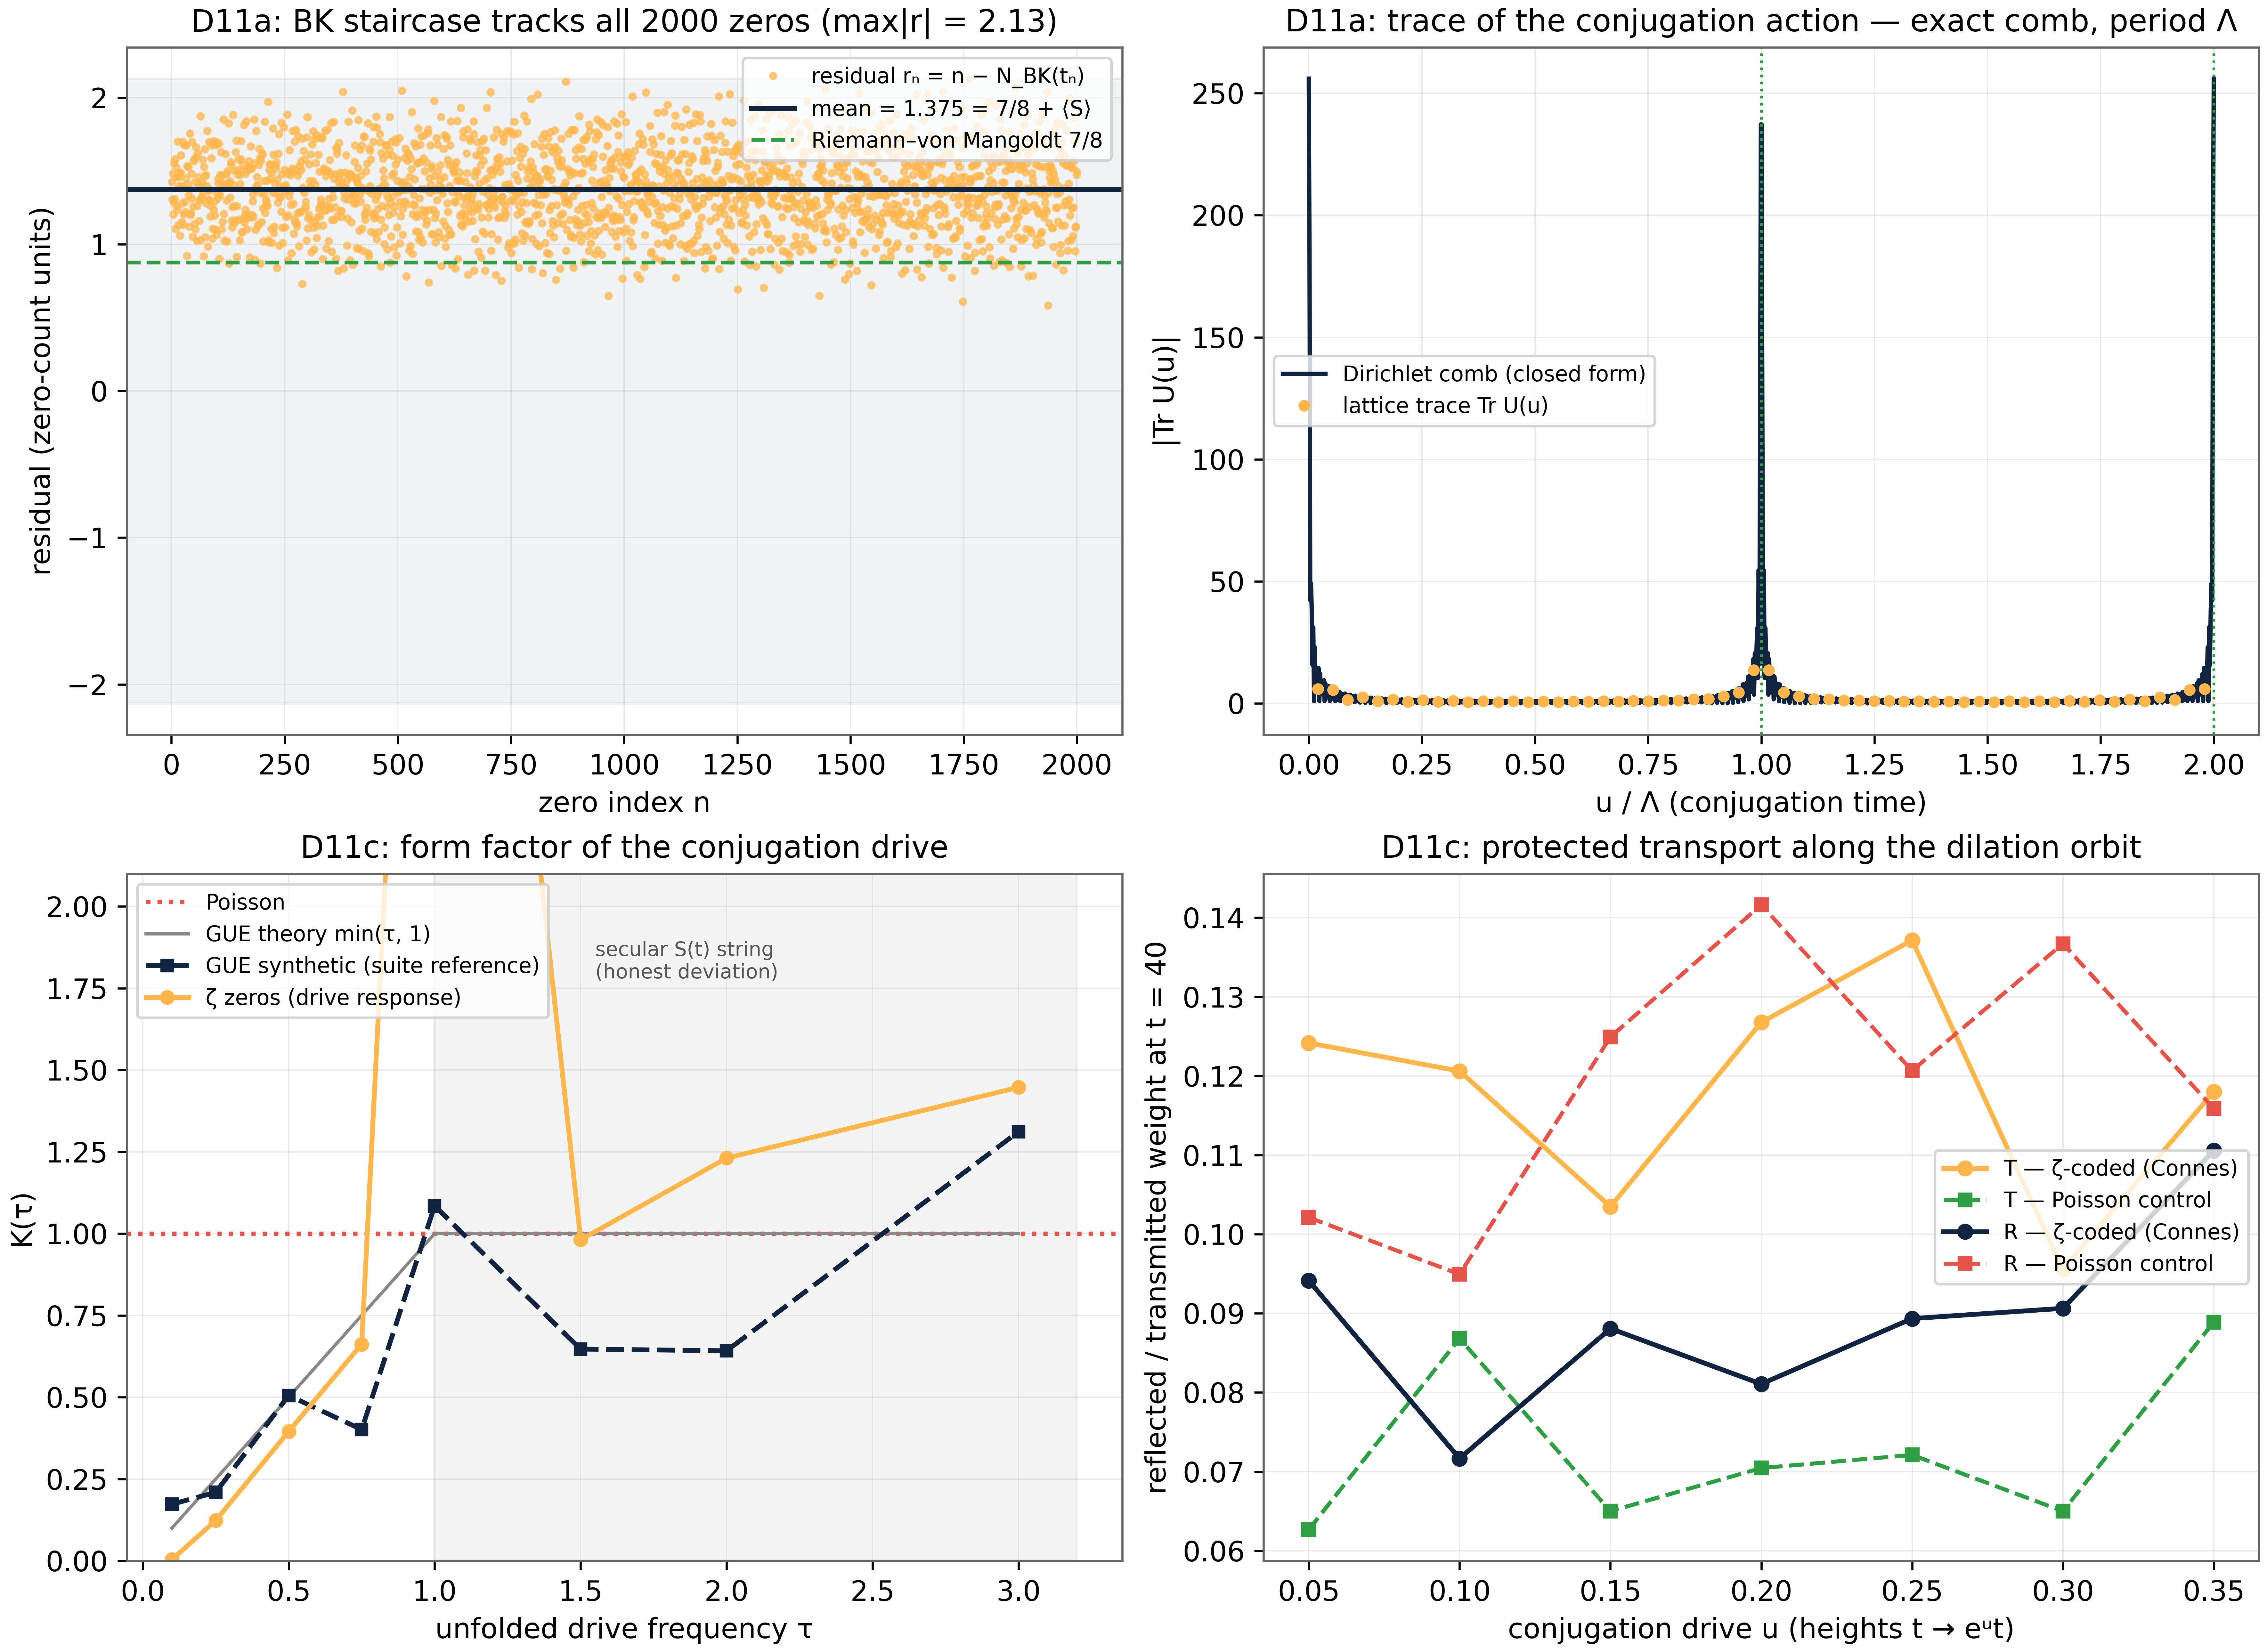
\includegraphics[max width=\columnwidth, max height=0.42\textheight]{figures/fig_D11_berry_keating.png}
\caption{Canonical D11 figure (600 dpi): the exact operator, the recognition identity and the drive form factor, produced by the original harness.}\label{fig:d11_1}
\end{figure}
\begin{figure}[htbp]\centering
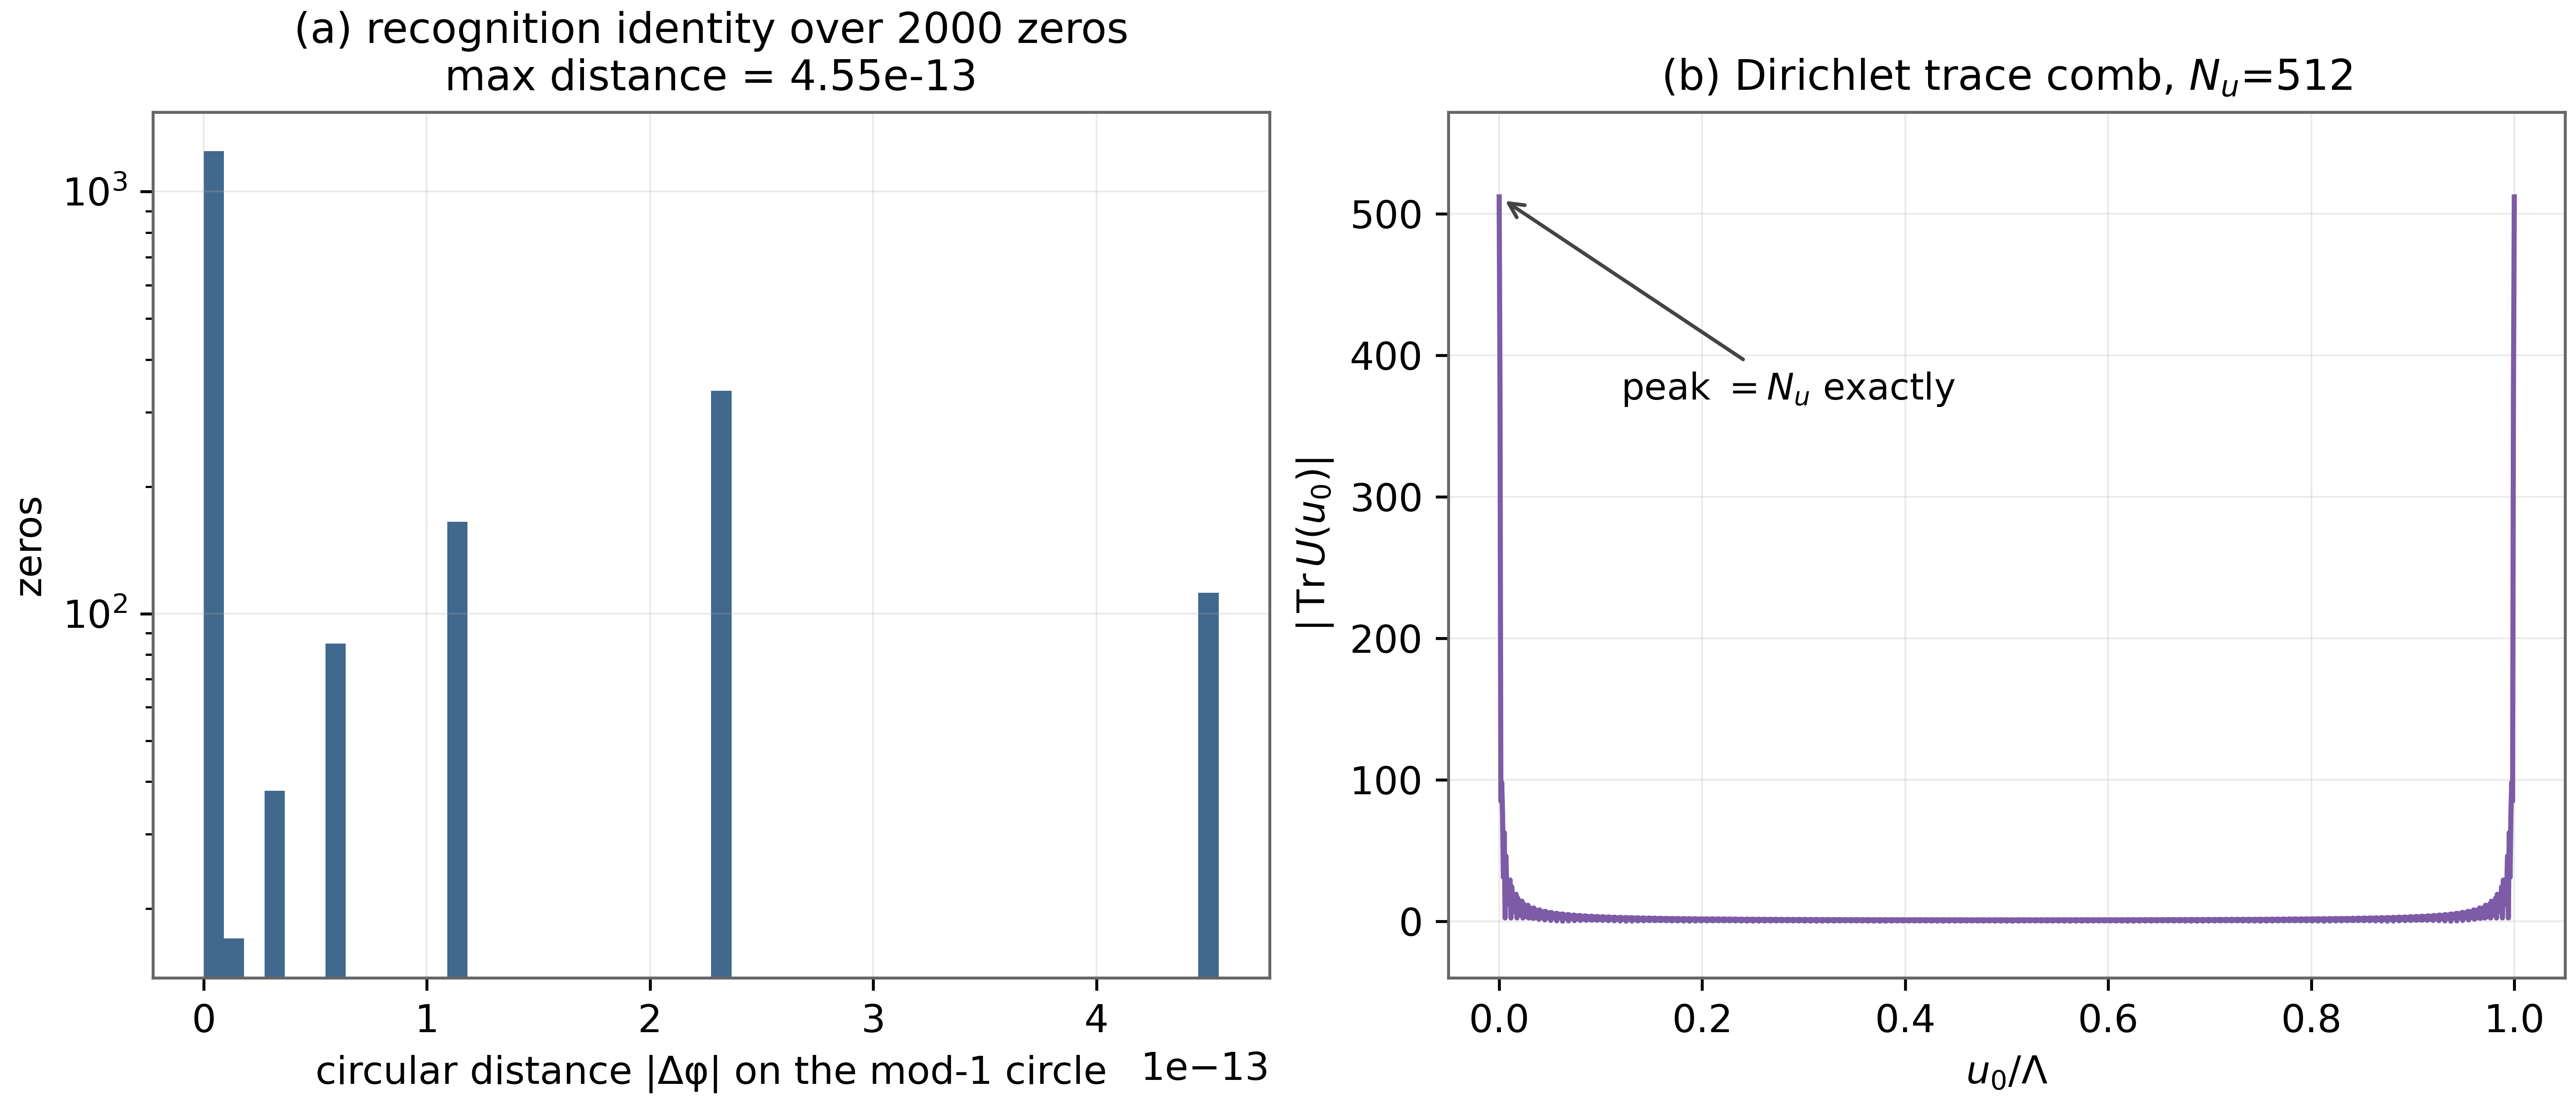
\includegraphics[max width=\columnwidth, max height=0.42\textheight]{figures/d11_extra_recognition_comb.png}
\caption{Companion panels (recomputed): (a) the recognition-identity circular-distance histogram over 2000 zeros (log scale; max $4.6\times10^{-13}$); (b) the Dirichlet trace comb $|\mathrm{Tr}\,U(u_0)|$ with the exact $N_u$ peak annotated.}\label{fig:d11_2}
\end{figure}

\section{Discussion}
D11 turns the laboratory from a Dirac-verifier into a zeta-arithmetic instrument: the same lattice now carries an exact conjugation-action operator, an identity connecting its coding to the Berry--Keating staircase, and a dynamical protection law that survives re-coding. The honest deviations -- the $\tau \ge 1$ string and the measured $\langle S\rangle$ offset -- are not noise but the expected finite-cutoff structure of the Connes framework, and they are documented as such \cite{connes,connesconsani}.

The natural continuations are precisely D12--D14: taking $N_u \to \infty$ at fixed density (the thermodynamic limit of the same comb), coupling the drive to the D9 wall (the conjugation acting on an index-bearing mode), and pushing the form factor to large heights where the plateau becomes exact. Each is realized in this laboratory and has its own companion monograph.

\section{Reproducibility}
\begin{itemize}[leftmargin=1.2em, itemsep=0.15em]
\item \textbf{Single test:} \texttt{python3} \path{code/dirac_lab_extensions2.py} \texttt{--test D11} (add \texttt{--quick} for a reduced pass; \texttt{--no-figures} to skip the 600-dpi figure).
\item \textbf{Canonical run:} \texttt{make all} regenerates the whole D1--D14 ledger into \path{results/}; this monograph's ledger is the verbatim per-check table of that run.
\item \textbf{Determinism:} seed 96 (parent convention); the $\zeta$ tables are the Odlyzko-derived files in \path{data/} with provenance in their headers.
\item \textbf{Figures:} the canonical figure was regenerated into this folder by the v1.4 harness (the original test function itself); companion panels are recomputed with the same modules (\path{scripts/make_extra_figures.py}). All figures are 600 dpi.
\item \textbf{Cross-verification:} \texttt{julia} \path{code/dirac_lab_cross_ext2.jl} re-derives the whole Berry--Keating operator block, 6/6 (ALL PASS).
\item \textbf{Artifacts in this folder:} \path{monograph.tex} (this document's source), \path{results.json} (machine-readable ledger), \path{figures/} (600-dpi figures), and the canonical CSV of the test.
\end{itemize}

\section*{References}
\begin{thebibliography}{99}\small
\bibitem{berrykeating} M. V. Berry and J. P. Keating, $H = xp$ and the Riemann zeros, in Supersymmetry and Trace Formulae (Kluwer, 1999), pp. 355--367.
\bibitem{connes} A. Connes, Trace formula in noncommutative geometry and the zeros of the Riemann zeta function, Selecta Math. (N.S.) 5, 29 (1999).
\bibitem{connesconsani} A. Connes and C. Consani, SPECTRA and the Riemann hypothesis, Int. J. Number Theory 14, 1247 (2018).
\end{thebibliography}

\vfill
\noindent\rule{\textwidth}{0.4pt}\\[0.2em]
{\footnotesize\color{labgray} AB-Cloud Dirac Laboratory · per-test monograph series v1.4 · compiled with Tectonic (LaTeX) · all numbers traceable to \texttt{results/run\_20261006\_full\_v13} · \texttt{D11} of 14.}

\end{document}